\section{Analisi Preliminare}\label{analisipre}

Il sito in analisi, \url{http://golarion.altervista.org/}, è un sito nato con l'obiettivo di
rendere di dominio pubblico, accessibile dal web, il materiale relativo al gioco di ruolo
cartaceo \href{https://it.wikipedia.org/wiki/Pathfinder_gioco_di_ruolo}{Pathfinder} della \emph{Paizo Publishing}. 
Infatti, gran parte del materiale del gioco è sotto la \emph{Open Game Licence} (OGL). Secondo Wikipedia:
\begin{quote}
    La OGL descrive due forme di contenuti: l'Open Gaming Content (OGC), ovvero il contenuto che 
    rappresenta le meccaniche di gioco, che viene distinto dal contenuto non-OGC, definito ``closed content'' 
    (in opposizione all'``open content''), protetto invece dalle normali norme sul copyright.    
\end{quote}

Il materiale non-OGC contiene prevalentemente materiale sull'ambientazione di gioco. \emph{Golarion} è una 
wiki che contiene perlopiù le meccaniche di gioco.

\subsection{Homepage e struttura del sito}
L'homepage è paragonabile alla \emph{vetrina} di un negozio, e ricopre un ruolo similare nel web.
La \emph{homepage} del sito si presenta come segue:

\begin{figure}[hbt]
    \centering
    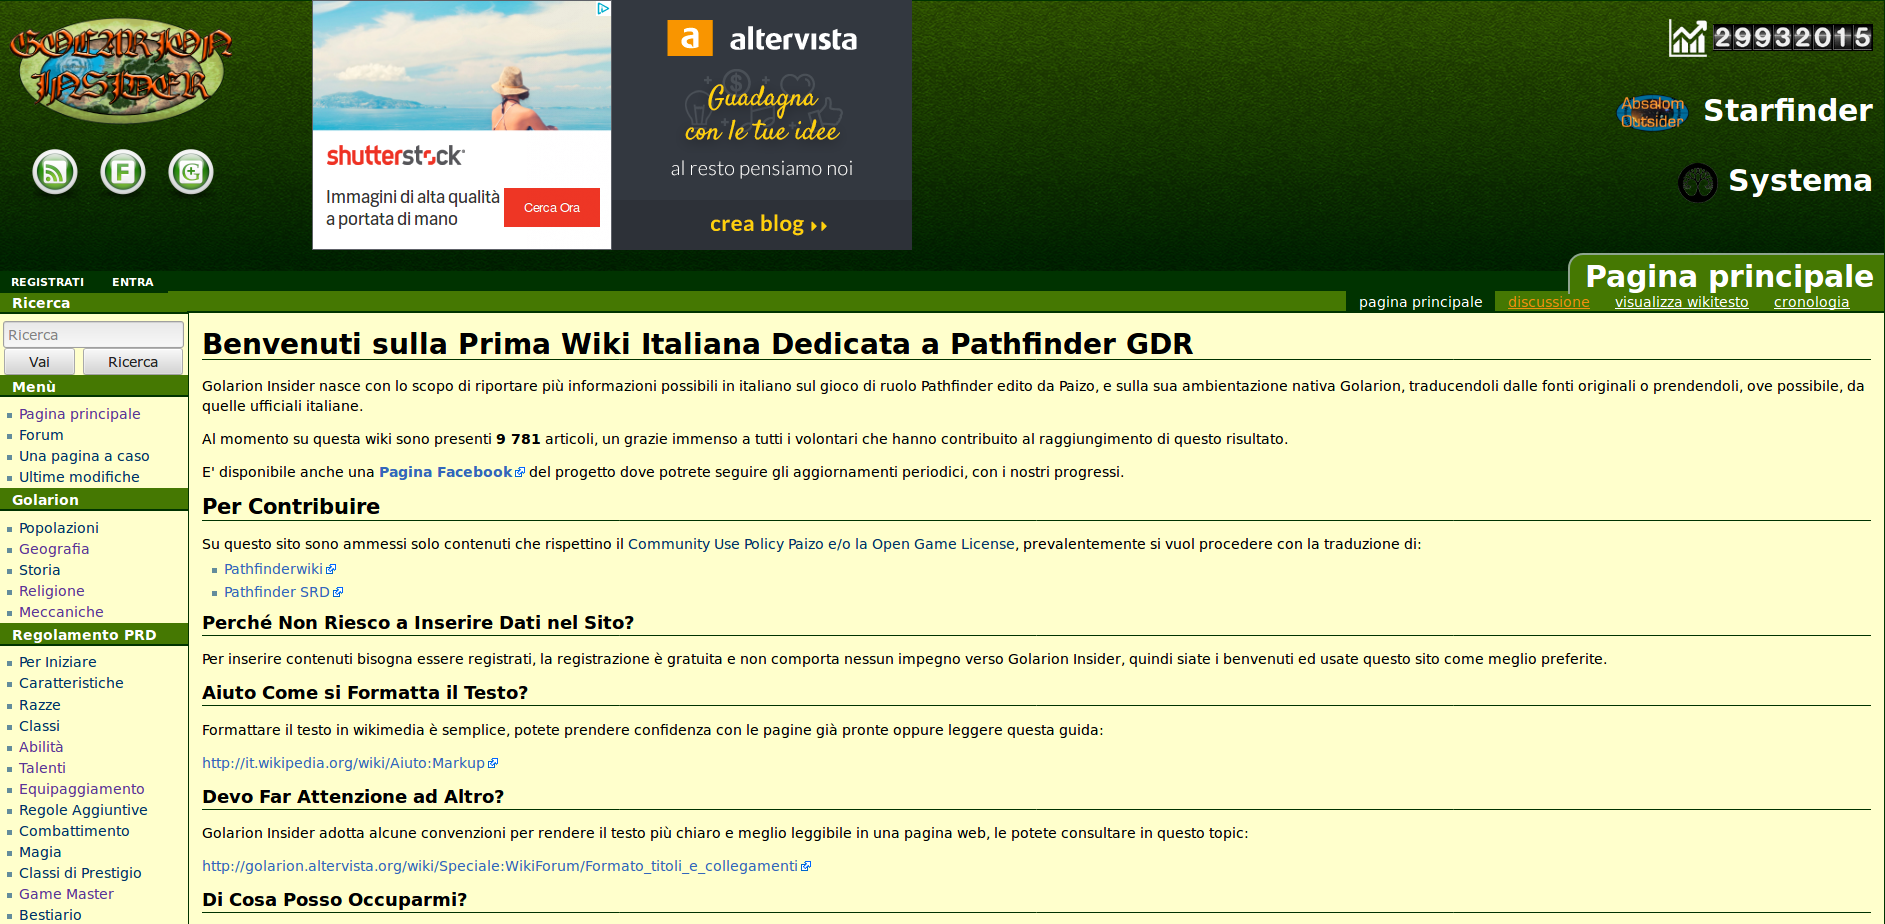
\includegraphics[width=\textwidth]{img/home.png}
    \caption{Homepage del sito.}
    \label{homepage}
\end{figure}

Come è possibile notare, dal menù si può ricavare una suddivisione del sito stesso in 4 macrosezioni:
\begin{itemize}[noitemsep]
    \item Menù;
    \item Golarion (l'ambientazione del gioco);
    \item Regolamento PRD;
    \item Strumenti (non visibile nell'immagine per ovvie ragioni).
\end{itemize}
Tuttavia, oltre a questo, è difficile ricavare una vera e propria suddivisione o struttura del sito. 
Si tratta perlopiù di \emph{hyperlinks} che mandano da una pagina all'altra del sito.

\paragraph{Analisi dell'homepage} L'homepage risulta poco attraente, per via dell'assenza di ogni tipo di multimedia
(che aiutano una homepage ad essere più apprezzata dall'utente) ma essendo un sito raggiunto da
un'utenza che sa già lo scopo della visita (quello di informarsi su un certo aspetto del gioco), non è molto rilevante. 
Per il resto, non presenta un'eccessiva mole di informazioni e c'è una buona suddivisione dei paragrafi, rendendo i 
titoli delle \emph{keywords}, cosa che aiuta a rilassare i timer del visitatore.\par 
Inoltre, la visita media non sarà caratterizzata dalla navigazione dalla homepage: si arriverà nella maggior parte 
dei casi tramite \emph{deep linking} dal proprio browser ad una pagina interna del sito (e.g. ricercando ``Attacco poderoso golarion''
su \texttt{Google}).